% !TEX root = main.tex
\section{Computational complexity and run-times of the evaluated Thompson sampling algorithms}
\label{asec:exec_times}
Computational cost is an important metric in real-life bandit scenarios, which motivated us to provide a computational analysis of our proposed algorithm in Section 3.2.2. As explained there, in general, the computational complexity is upper bounded by $\mathcal{O}(T \cdot Gibbs_{steps})$, which depends on the convergence criteria: \ie either the model likelihood of the sampled chain is stable within an $\epsilon$ likelihood margin between steps, or a maximum number of iterations $Gibbs_{max}$ is reached. As such, tweaking these two values controls the resulting run-times.

We provide below a comparison of the run-times incurred in the set of experiments described in the manuscript, for which we would like to raise two cautionary disclaimers:
\begin{itemize}
	\item We compare \textbf{algorithms with different implementations}: \\
	The proposed \texttt{Nonparametric TS} is implemented with standard python libraries (\ie numpy, scipy), while the rest of the algorithms are implemented in Tensorflow, as provided in the \href{https://github.com/tensorflow/models/tree/master/research/deep_contextual_bandits}{Deep Contextual bandit implementation} by~\citet{ip-Riquelme2018}. Our goal here is to introduce a new bandit algorithm, and improving the efficiency of our implementation (or coding it in Tensorflow) is out of the scope of this work.
	\item Both our algorithm and those in the \href{https://sites.google.com/site/deepbayesianbandits/}{deep contextual bandits showdown} require \textbf{updates at every time instant that depend on the number of observations per-arm $t_a$}:\\
	Performance and running-time differences can be achieved if one tweaks each algorithm's settings for model updates. As explained in~\cite{ip-Riquelme2018}, a key question is how often and for how long models are updated, as these will determine their running-times in practice. Even if ideally, one would like to re-train models after each new observation (and for as long as possible), this may limit	the applicability of the algorithms in online scenarios. In this work, we have executed all baselines based on the default hyperparameters suggested by~\citet{ip-Riquelme2018} ---which limits the retraining process per interaction to 100 epochs, upper bounding the execution time per bandit interaction--- and argue that tweaking the hyperparameters of such algorithms to reduce running-times is out of the scope of this work.
\end{itemize}

Nevertheless, and as illustrative examples, we show in Figure~\ref{afig:mixture_scenarios_bandit_showdown_exec_times} the running times of all algorithms (averaged across realizations).
First, we note that \texttt{LinearGaussian TS}, due to its conjugacy-based posterior updates that can be computed sequentially, is the fastest algorithm in all scenarios.
Second, we observe that the algorithms in~\cite{ip-Riquelme2018} have a similar running-time across all scenarios, expected due to the suggested configuration that limits per-interaction run-time to 100 epochs.
Third, the run-times of our \texttt{Nonparametric TS} algorithm vary across scenarios, as updating the nonparametric posterior model takes more or less time depending on the complexity of the true reward model: it shows low computational complexity in linear Gaussian scenarios, while incurring in higher computational cost when fitting the most challenging \texttt{Scenarios B, C}, and \texttt{D}.
However, as demonstrated in Figures~\ref{afig:scenario_A_exec_times},~\ref{afig:scenario_B_exec_times},~\ref{afig:scenario_C_exec_times} and~\ref{afig:scenario_D_exec_times}, we can drastically reduce the run-time of \texttt{Nonparametric TS} by upper-bounding the number of Gibbs iterations, yet achieve satisfactory performance, as demonstrated in Figure~\ref{fig:mixture_scenarios_bandit_showdown_gibbsmaxiter} of the manuscript.

\begin{figure*}[!h]
	\centering
	\begin{subfigure}[c]{0.45\textwidth}
		\includegraphics[width=\textwidth]{./figs/linear_showdown/exec_time_barplot}
		\vspace*{-5ex}
		\caption{Contextual linear Gaussian MAB.}
		\label{afig:linear_showdown_exec_times}
	\end{subfigure}
	\begin{subfigure}[c]{0.45\textwidth}
		\includegraphics[width=\textwidth]{./figs/sparse_linear_showdown/exec_time_barplot}
		\vspace*{-5ex}
		\caption{Contextual sparse linear Gaussian MAB.}
		\label{afig:sparse_linear_showdown_exec_times}
	\end{subfigure}
	\vspace*{-2ex}
	\caption{Mean run-time (standard deviation shown as error bars) in seconds for $R=500$ realizations  of the studied methods in linear contextual multi-armed bandits.}
	\label{afig:contextual_bandit_showdown_exec_times}
\end{figure*}

\begin{figure*}[!h]
	\centering
	\begin{subfigure}[c]{0.45\textwidth}
		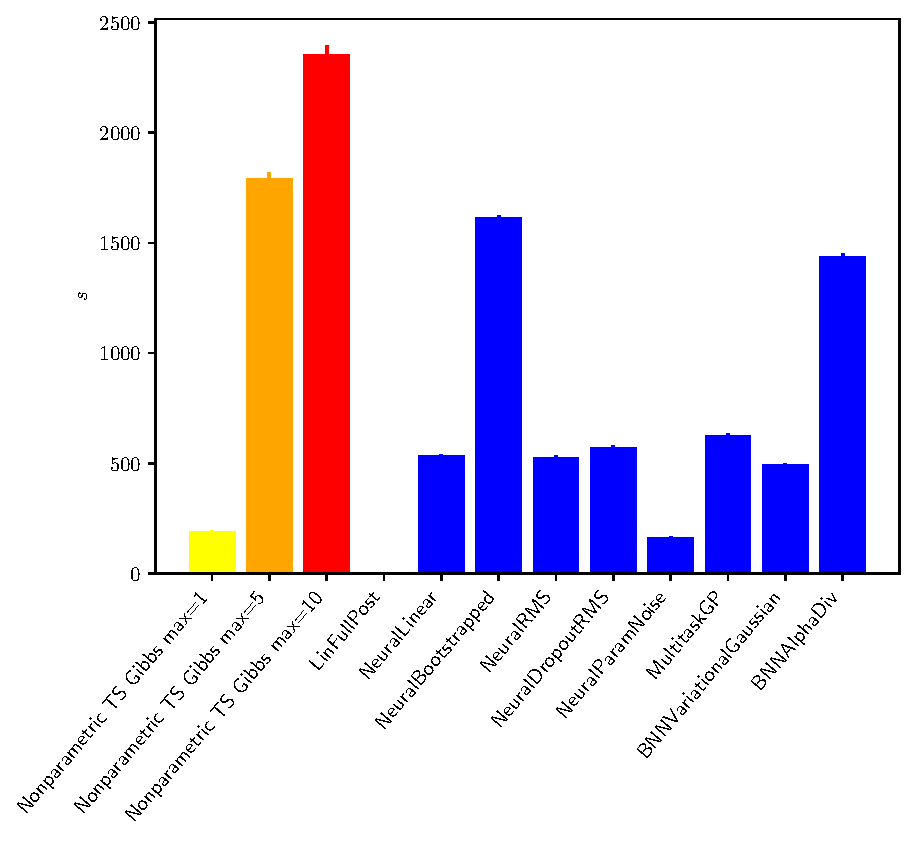
\includegraphics[width=\textwidth]{./figs/linear_gaussian_mixture_easy/exec_time_barplot}
		\vspace*{-5ex}
		\caption{\texttt{Scenario A}.}
		\label{afig:scenario_A_exec_times}
	\end{subfigure}
	\begin{subfigure}[c]{0.45\textwidth}
		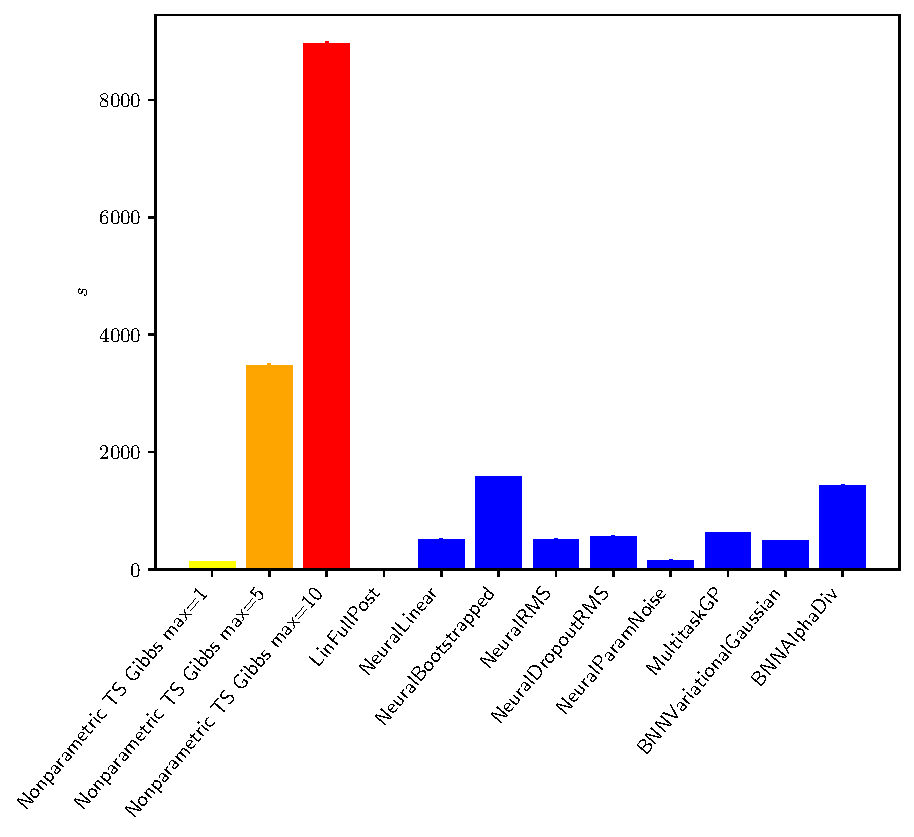
\includegraphics[width=\textwidth]{./figs/linear_gaussian_mixture_hard/exec_time_barplot}
		\vspace*{-5ex}
		\caption{\texttt{Scenario B}.}
		\label{afig:scenario_B_exec_times}
	\end{subfigure}
	
	\begin{subfigure}[c]{0.45\textwidth}
		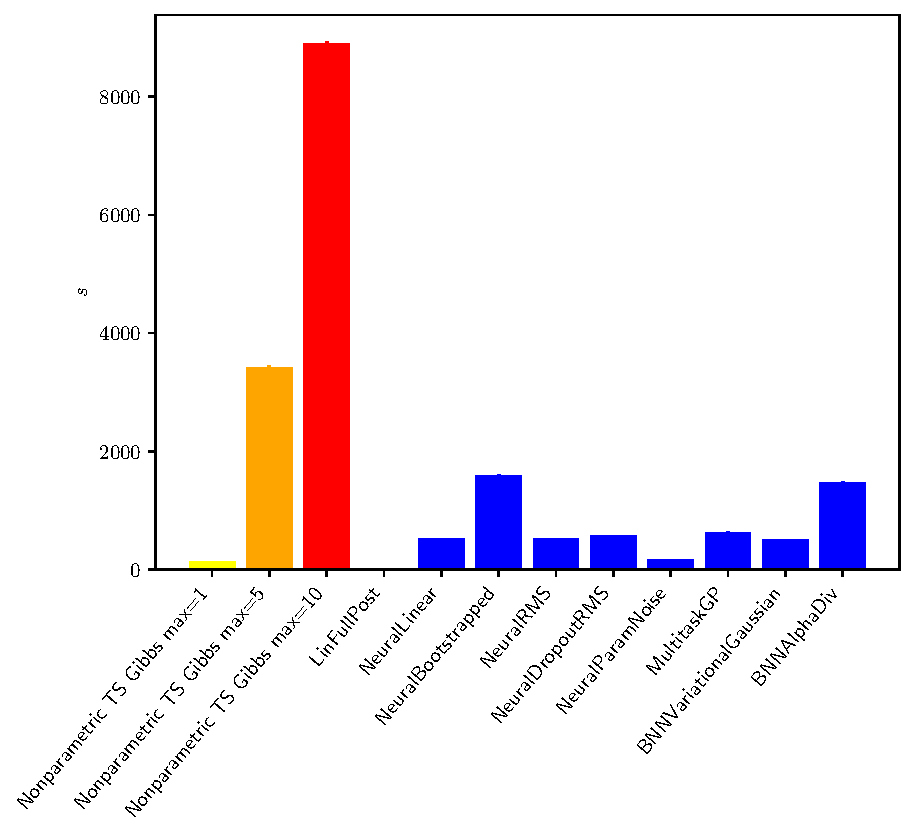
\includegraphics[width=\textwidth]{./figs/linear_gaussian_mixture_unbalanced/exec_time_barplot}
		\vspace*{-5ex}
		\caption{\texttt{Scenario C}.}
		\label{afig:scenario_C_exec_times}
	\end{subfigure}
	\begin{subfigure}[c]{0.45\textwidth}
		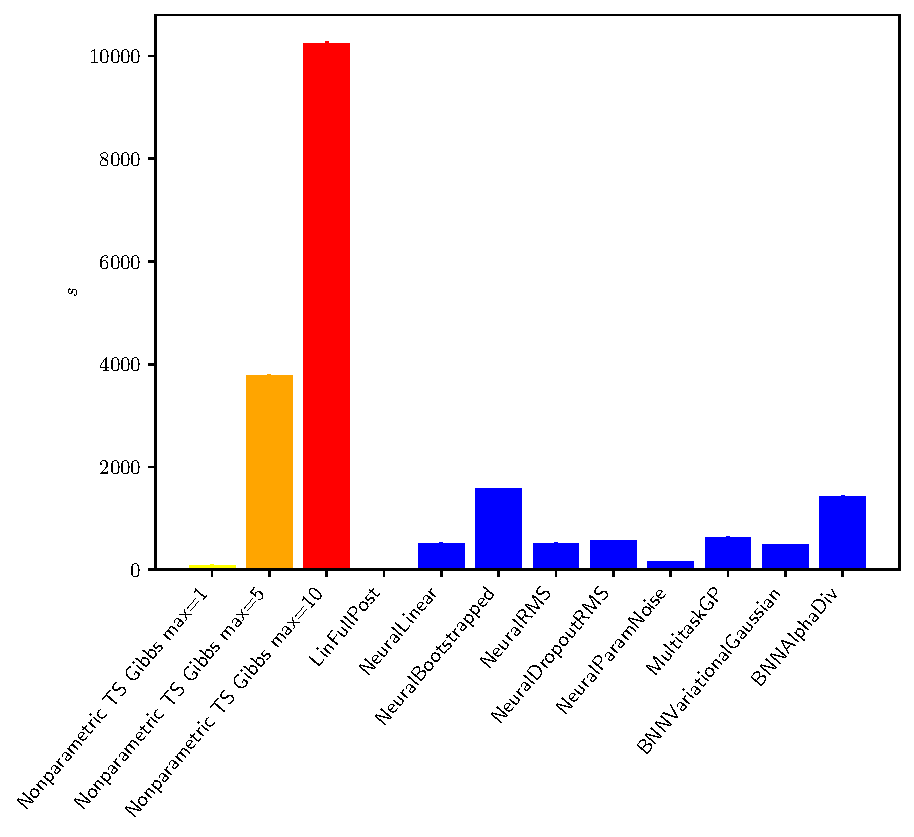
\includegraphics[width=\textwidth]{./figs/linear_gaussian_mixture_heavy_tail/exec_time_barplot}
		\vspace*{-5ex}
		\caption{\texttt{Scenario D}.}
		\label{afig:scenario_D_exec_times}
	\end{subfigure}
	\vspace*{-2ex}
	\caption{Mean run-time (standard deviation shown as error bars) in seconds for $R=500$ realizations  of the studied methods in all scenarios.}
	\label{afig:mixture_scenarios_bandit_showdown_exec_times}
\end{figure*}

We conclude by reiterating that, in general, we recommend to run the algorithm until full convergence, but suggest to limit the number of Gibbs iterations as a practical recommendation with good empirical regret performance ---analogous to the suggestion by~\citet{ip-Riquelme2018} to limit the number of per-iteration epochs for neural network based algorithms.
